\begin{thm}{140}{\hosi 4}{大阪市大理系 (2017) 改}
 半径1の円柱を、底面の直径を含み、底面と角$\alpha (0<\alpha<\dfrac{\pi}{2})$ をなす平面で切ってできる小さい方の立体$K$を考える。ただし、円柱の高さは十分大きいとする。$K$の体積$V$と表面積$S$を求めよ。
\end{thm}

\begin{figure}[H]
 \centering
 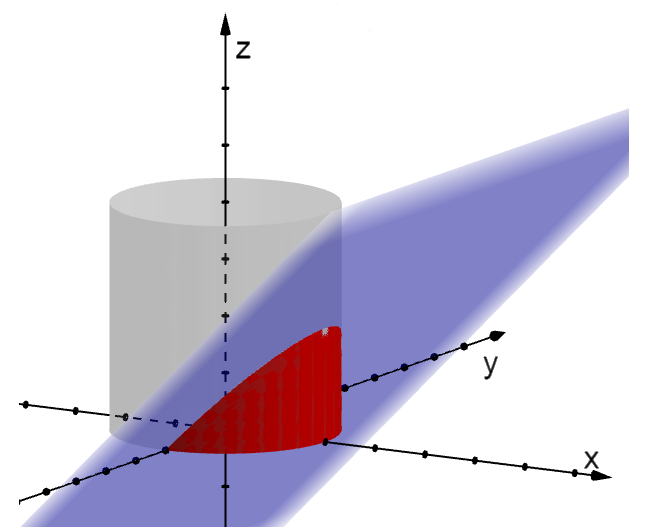
\includegraphics[width=0.7\linewidth]{../problems/Q_140/A_140.png}
\end{figure}
上図のように座標軸を設定し、平面$y=k$ (ただし$-1\le k\le 1$)における断面を考える。これは直角三角形で、底辺は$\sqrt{1-y^2}$であり、底辺と斜辺のなす角は$\alpha$となる。この三角形の面積$T(y)$は、
\begin{align*}
 T(y)&=\frac{1}{2}\tan\alpha (1-y^2)
\end{align*}
これを積分することで体積が得られる。
\begin{align*}
 V&=\int_{-1}^1\! \frac{1}{2}\tan\alpha (1-y^2) \,dy \\
 &=\tan\alpha\Bigl[y-\frac{1}{3}y^3\Bigr]_0^1=\frac{2}{3}\tan\alpha
\end{align*}

表面積を構成するものは、半径1の半円 (底面)、2つの軸半径がそれぞれ1, $\dfrac{1}{\cos\alpha}$の楕円の半分 (平面による断面)、円柱の側面の一部である。半円の面積は$\dfrac{\pi}{2}$、楕円の半分の面積は$\dfrac{\pi}{2\cos\alpha}$である。$x$軸と角$\theta$をなし$xy$平面と鉛直な面での断面を考えると、これは直角三角形で、高さは$\tan\alpha\cos\theta$ となる。この直角三角形の高さを$-\dfrac{\pi}{2}\le\theta\le\dfrac{\pi}{2}$で積分すると側面積になって\footnote{$y=k$での断面の周を積分すると、積分の向きと側面の向きが異なるため、正しい側面積が得られない。}、
\begin{align*}
 \int_{-\frac{\pi}{2}}^{\frac{\pi}{2}}\!\tan\alpha\cos\theta\,d\theta=\tan\alpha\Bigl[\sin\theta\Bigr]_{-\frac{\pi}{2}}^{\frac{\pi}{2}}=2\tan\alpha
\end{align*}
である。これらから表面積は、
\[ S=\frac{\pi}{2}+\frac{\pi}{2\cos\alpha}+2\tan\alpha \]
